% ----------------------------------------------------------------
% Initial Packages
% 
% Refs:
% https://github.com/schnorr/infufrgs/blob/master/exemplos/cic-tc.tex

% Use unicode
\usepackage[utf8]{inputenc}   % pacote para acentuação

% Necessário para incluir figuras
\usepackage{graphicx}         % pacote para importar figuras
\usepackage{svg}

\usepackage{times}            % pacote para usar fonte Adobe Times
% \usepackage{palatino}
% \usepackage{mathptmx}       % p/ usar fonte Adobe Times nas fórmulas

\usepackage[alf,abnt-emphasize=bf]{abntex2cite}	% pacote para usar citações abnt

% ----------------------------------------------------------------
% Other Custom Packages
% 

\usepackage{csquotes}
\usepackage{hyperref}
\usepackage{subcaption}
\usepackage{float}
\usepackage{blindtext}

% ----------------------------------------------------------------
% Code Listings
% 
% Provided by Alexandre Ilha (MSc Thesis)
% 
% Refs:
% https://en.wikibooks.org/wiki/LaTeX/Source_Code_Listings
% https://ctan.org/pkg/listings
% https://mirrors.ctan.org/macros/latex/contrib/listings/listings.pdf
\usepackage{listings}

\lstdefinelanguage{P4}[]{C++}{
    morekeywords={accept, action, actions, apply, bit, const, control, default, default_action, header, in, inout, key, out, packet_in, parser, select, size, start, state, struct, table, transition}
}

\lstdefinelanguage{Zeek}[]{C++}{
    morekeywords={addr, const, count, event, export, global, local, module, port, print, priority, redef, timeout, when},
    morecomment=[l]{\#}
}

\lstdefinelanguage{Bash}[]{}{
    morekeywords={},
    morecomment=[l]{\#},
    moredelim=[is][\bfseries]{<@}{@>}
}

\lstdefinelanguage{Py}[]{Python}{
    morecomment=[s]{"""}{"""},
    morekeywords={self}
}

\lstdefinestyle{code}{
    breaklines,
    basicstyle=\ttfamily\scriptsize,
    captionpos=t,
    floatplacement=htb,
    frame=tb,
    keywordstyle=\bfseries,
    numbers=left,
    numbersep=5pt,
    numberstyle=\ttfamily\tiny,
    showspaces=false,
    showstringspaces=false,
    tabsize=2
}

\lstdefinestyle{p4}{
    style=code,
    language=P4
}

\lstdefinestyle{zeek}{
    style=code,
    language=Zeek
}

\lstdefinestyle{bash}{
    style=code,
    language=Bash
}

\lstdefinestyle{python}{
    style=code,
    language=Py
}

\lstdefinestyle{cpp}{
    style=code,
    language=C++
}

\lstdefinestyle{inline}{
    breaklines,
    basicstyle=\ttfamily\normalsize
}

\lstset{style=code}

\newcommand{\code}[1]{\texttt{#1}}
% TODO figure out why this messes up line breaks.
% \renewcommand{\code}[1]{\lstinline[style=inline]{#1}}

% ----------------------------------------------------------------
% Custom name and simple definitions
%
% ----------------------------------------------------------------
% Definitions of names that haven't been decided yet:
% 

\newcommand{\TheSolutionName}[0]{ZPO}
\newcommand{\TheCodeGeneratorName}[0]{Zeek-P4 Offloader}

\newcommand{\Offloader}[0]{Offloader}
\newcommand{\Offloaders}[0]{Offloaders}

\newcommand{\ProtocolTemplate}[0]{Protocol Template}
\newcommand{\ProtocolTemplates}[0]{Protocol Templates}

\newcommand{\zeekconn}[0]{\textit{Connection}}

% ----------------------------------------------------------------
% Definitions to make sure some words are standard
% 

\title{A Code Generation Tool and Architecture for enabling Intrusion Detection Systems at Data Planes Speeds}
\author{Sonntag Hagen}{Lucas}
\advisor[Prof.~Dr.]{Paschoal Gaspary}{Luciano}
\coadvisor[MSc.]{da Silveira Ilha}{Alexandre}
\date{July}{2022}
\location{Porto Alegre}{RS}

\begin{document}

\keyword{Zeek}

\maketitle

\chapter*{Acknowledgements}

Acknowledgements...

\chapter*{Agradecimentos}

Agradeço aos meus pais Rejane Sonntag Hagen e Roberto Hagen por me proporcionarem uma educação de qualidade e me apoiarem em todos os momentos. Ao meu irmão Bruno e minha namorada Giulia que fizeram parte dessa trajetória, incentivando-me a seguir em frente e a não desistir.

Ao meu orientador, Prof.~Dr.~Luciano Paschoal Gaspary, que me guiou nessa árdua tarefa chamada TCC, sempre com paciência e sabedoria, compartilhando um pouco de todo o seu conhecimento e sua experiência. Ao doutorando MSc.~Jonatas Adilson Marques e ao MSc.~Alexandre da Silveira Ilha por compartilharem seu tempo sanando as minhas dúvidas e guiarem-me em minha pesquisa.

Agradeço também à intituição UFRGS e seus professores, onde iniciei uma jornada profissional, conheci grandes amigos e construí meu currículo. Sou imensamente grato por todas as oportunidades recebidas. Faço aqui menção dos professores Raul e Taisy Weber, Lucas Schnorr e Gabriel Nazar os quais tiverem um participação especional nessa jornada acadêmica.

Além disso, gostaria de agradecer aos meus amigos e colegas de curso, os quais foram muito importantes em minha trajetória acadêmica. Meciono, em especial, meus colegas de intercâmbio Bernardo, Emily e Iron, os quais se tornaram uma família no ano de 2020, durante o auge da Pandemia da COVID-19. Ainda no intercâmbio, agredeço ao meu orientador Prof.~Dr.~Reinhard Gotzhein e ao doutorando MSc.~Paulo Aragão, que me acolheram e mentoraram a minha passagem pela Technische Universität Kaiserslautern. 

Ademais, gostaria de mencionar os meus chefes de estágios e outros colegas de trabalho, com os quais dividi momentos de apredizado e de lazer: Lauro Souza e Breno Araújo, do estágio que realizei no Google Brasil no ano de 2021-2022; Daniel Thiel, Hélio Fuques e Hernandi Krames do estágio na AEL Sistemas no ano de 2018-2020.

Por fim, agradeço aos demais professores, mentores, familiares e amigos, que direta e indiretamente participaram da minha jornada acadêmica, transmitindo aprendizados, compatilhando ideias e bons momentos, dividindo momentos de angústia e também de alegria.

\clearpage

% palavras-chave
% iniciar todas com letras minúsculas, exceto no caso de abreviaturas

% Keywords precisam estar definidos ANTES do \maketitle

\begin{abstract}
Abstract....
\end{abstract}

\begin{englishabstract}
{TITULO EM PORTUGUES}
{palavras chaves}

Abstract em Portugues...


\end{englishabstract}




\listoffigures
\listoftables
% lista de abreviaturas e siglas
% o parametro deve ser a abreviatura mais longa

\begin{listofabbrv}{FPGA}
    \item[API]  Application Programming Interface
    \item[ARP]  Address Resolution Protocol
    \item[ASIC] Application-Specific Integrated Circuit
    \item[AST]  Abstract Syntax Tree
    \item[BMv2] Behavioral Model Version 2
    \item[C2]   Command and Control
    \item[DDoS] Distributed Denial of Service
    \item[DDR]  Double data rate
    \item[DoS]  Denial of Service
    \item[DPD]  Dynamic Protocol Detection
    \item[DSL]  Domain-specific Language
    \item[EE]   Zeek Event Engine
    \item[FPGA] Field Programmable Gate Array
    \item[FTP]  File Transfer Protocol
    \item[ICMP] Internet Control Message Protocol
    \item[IDS]  Intrusion Detection System
    \item[IP]   Internet Protocol
    \item[IPv4] Internet Protocol Version 4
    \item[IPv6] Internet Protocol Version 6
    \item[MT/s] Megatransfers per Second
    \item[NIDS] Network Intrusion Detection System
    \item[NPU]  Network Processing Unit
    \item[NTP]  Network Time Protocol
    \item[NVMe] Nonvolatile Memory Express
    \item[PAF]  Packet Analysis Framework
    \item[PCAP] Packet Capture
    \item[PDP]  Programmable Data Plane
    \item[PDU]  Protocol Data Unit
    \item[PFD]  Programmable Forwarding Device
    \item[POF]  Protocol Oblivious Forwarding
    \item[PPS]  Packets Per Second
    \item[PSI]  Zeek Policy Script Interpreter
    \item[RAM]  Random Access Memory
    \item[RNA]  Reconfigurable Network Analytics
    \item[RQ]   Research Question
    \item[SDN]  Software Defined Network
    \item[SDN]  Software Defined Network
    \item[SSD]  Solid State Drive
    \item[TCP]  Transmission Control Protocol
    \item[TTL]  Time-To-Live
    \item[UDP]  User Datagram Protocol
    \item[UID]  Unique Identifier
    \item[VoIP] Voice over Internet Protocol
\end{listofabbrv}


% lista de símbolos
% \begin{listofsymbols}{$\alpha\beta\pi\omega$}
%       \item[$\sum{\frac{a}{b}}$] Somatório do produtório
%       \item[$\alpha\beta\pi\omega$] Fator de inconstância do resultado
% \end{listofsymbols}

\tableofcontents

     % 10+
\chapter{Introduction}
\label{cap:introduction}

Introduction...

\section{Motivation}

% \section{Threat Model}
% Not sure where this section goes... leaving it here so we don't forget.
    % 2
\chapter{Background}
\label{cap:background}

% Maybe use "Background and State of the Art"


\section{Zeek}
\label{sec:bg:zeek}


% TODO: don't forget to explain this from chapter 3:
% It consists of two high-level components: the RNA Host Engine, which executes in one of Zeek's worker nodes inside the IDS cluster;

Zeek is a.... \cite{AboutZeek}

Zeek started as Bro, which was proposed by Paxson \cite{Paxson1999}.

\subsection{Packet Capture}

\subsection{Event Engine}
\label{sec:bg:zeek_ee}

\subsection{Packet Analysis Framework}
\label{sec:bg:zeek_packet_analysis}

\subsection{Policy Script Analyzer}
\label{sec:bg:zeek_psi}

% Alexandre Ilha: TODO Explain in Ch. 2 that Zeek's PSI is an event-driven mechanism.


\subsection{Candidate Operations for Offloading}
\label{sec:bg:zeek_candidate_operations}

\section{Programmable Data Plane}
\label{sec:bg:pdp}

\subsection{P4}
\label{sec:bg:p4}
      % 5
\chapter{\TheSolutionName{}}
\label{cap:proposal}

In this chapter, we propose the \TheSolutionName{}, a solution for offloading some of Zeek's operations discussed in Section \ref{sec:candidate_operations} to Network Programmable Forwarding Devices compatible with P4. This proposal uses the Reconfigurable Network Analytics (RNA) architecture, which was initially proposed by Ilha \cite{Ilha2022}. Since \TheSolutionName{} also contributed to RNA's development, this text describes and presents them together.

\begin{figure}[h]
    \caption{RNA Framework - High-level architectural view}
    \begin{center}
        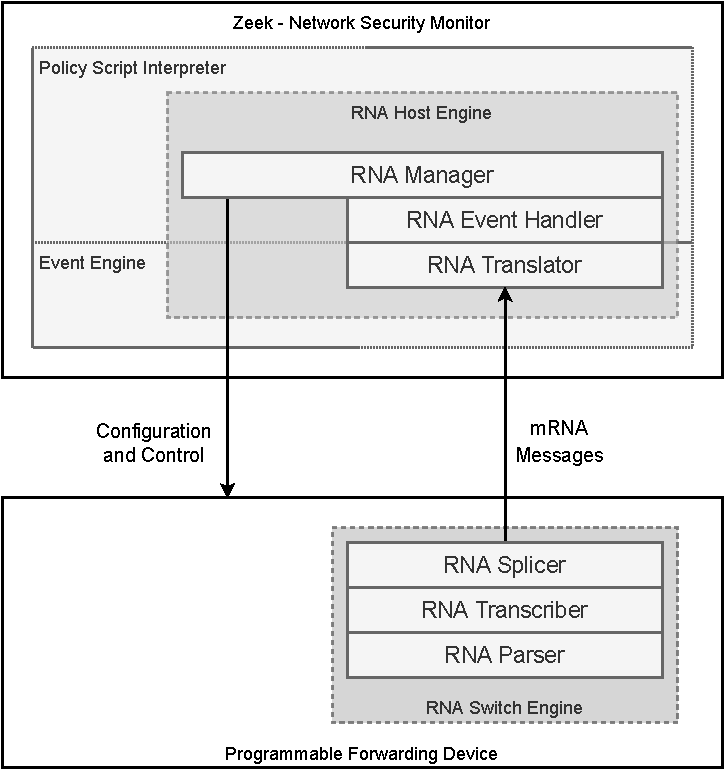
\includegraphics[width=0.7\textwidth]{images/arch_high_level.pdf}  
    \end{center}
    \label{fig:arch_high_level}
    \legend{Source: the author, adapted from Ilha \cite{Ilha2022}}
\end{figure}

Figure \ref{fig:arch_high_level} illustrates the RNA architecture. It is composed of two high-level components: the RNA Host Engine, which executes in one of Zeek's work nodes inside the IDS; and the RNA Switch Engine, which is executed in a P4 switch. Both components work together to offload packet analysis from Zeek to a programmable forwarding device. The RNA Switch Engine is able to better parse packets and identify some of their characteristics, which are then summarized and sent to the RNA Host Engine. This summarized message is called mRNA. When the IDS receives this message, it is first processed by our Host Engine. It then converts the summarized message into Zeek's native structures, which can then be forwarded to Zeek's normal processing pipeline. This procedure allows us to bypass some operations that would be costly, and deliver this information one step closer to the Policy Script Interpreter (PSI, Section \ref{sec:zeek_psi}), without disturbing its flow. By doing so, we make it that no change is required on existing scripts running on the PSI.

% TODO: check what to call this "'custom software' to be executed both...."
In the original concept of RNA, depending on the IDS scripts chosen to be monitored by the operator, it is necessary to develop custom software to be executed both by the Host Engine and the Switch Engine. This ad-hoc development process quickly becomes impractical when we increase the number of desired scripts to be offloaded. For this reason, later propose an automatic code generation tool, which allows \TheSolutionName{} to be a modular solution, where new offloaded scripts can be added or removed, without the need to develop new software. Before detailing this automated process, first, we revisit the architectural concepts.

% ==============================================================================
%                               RNA OVERVIEW
% ==============================================================================
\section{Overview}

In this section, we'll describe the components shown in Figure \ref{fig:arch_high_level}. We start with the RNA Host Engine, since it is the controlling part of the whole deployment, and then we describe the RNA Switch Engine.


% TODO: check if we'll remove the "RNA Event Handler" completely, or say it was removed but exists in the original RNA
The \textbf{Host Engine} unfolds into three components. The \textbf{RNA Manager} is a Zeek Script, which first configures the P4 switch, setting up a monitoring session and loading all P4 code that is required to execute the offloaded tasks. After configuring the switch, it registers all RNA Translators (one per-protocol of interest), so they receive mRNA messages. The \textbf{Translators} wait for such messages and translate them to Zeek native structures. Those structures are then used to trigger events, which are then consumed by the running scripts.

% % Removed: too much 'unwanted' information
% In order not to override and disturb the existing Zeek Packet and Protocol Analyzers described in Section \ref{sec:packet_analysis_framework}, the Translators are registered using a different protocol, the RNA protocol, which is used by the mRNA message (Section \ref{sec:mrna_message}) and is built over Ethernet. This means the packets encoded as mRNA messages, even if they represent an ICMP event, for example, will be first analyzed by the Ethernet \textit{Analyzer}, then the RNA Translator \textit{Analyzer}, where the normal flow for an ICMP packet would be the following analyzers: Ethernet, IPv4, and ICMP.

The \textbf{RNA Switch Engine} is the program that executes in our P4-compatible programmable forwarding device. It has three components and we'll be following the route of an incoming packet to explain them. The first component that processes a packet is the \textbf{RNA Parser}. It parses and extracts headers from each protocol, from the link layer, up to the application layer if required. After all headers have been extracted, the packet enters P4's ingress pipeline, where the \textbf{RNA Transcriber} is executed. It extracts useful information from the packet and sets metadata that later will be used to build our summarized message, while also filtering some undesired packets. Having all the required metadata and going into P4's egress pipeline, the \textbf{RNA Splicer} builds and sends our summarized message, the mRNA, to the Host Engine with all information it may require to trigger a native Zeek Event.

Another important structure to be explained is The \textbf{mRNA Message} is a summary of a packet, summarizing all the information that the Switch Engine was able to extract from it. Sending an mRNA message is better than sending the whole packet because the original packet contains a lot of headers that still would need to be parsed, a lot of information that is not necessary in some cases, and is not validated. In the summarized message, all information from L2 up to the L7 layer is gathered, filtered, and even formatted sometimes to a one-to-one translation to Zeek's native structures, saving Zeek from doing these operations on its own. The information-gathering process still needs to happen, but it does in the Switch Engine, which runs in a purpose-built device, making it much more efficient for this task. So the more information the switch is able to extract, the less Zeek has to do.

In an ideal world scenario, we would like to extract all information that Zeek needs to trigger an event, but sometimes that's not possible. Zeek's internal structures track a lot of connection states and use a lot of heuristics, which because of P4's limited processing power for general tasks, we are unable to implement. This requires the mRNA message to be modular, allowing us to send, together with it, a part of the packet that was not able to be processed in the switch. This ensures P4 extracts all information it can, leaving the rest for Zeek to finish analyzing.

% ==============================================================================
%                               RNA DETAILED ARCHITECTURE
% 
%  This includes modifications made to allow code generation
% ==============================================================================
\section{Detailed Architecture}

The \TheSolutionName{} was based on the RNA architecture, with the addition of modules that could be added and removed as the network operator wants to offload different scripts. Before explaining the inner details of the architecture, we will introduce two concepts that are fundamental for its understanding and will serve as inputs later for our code generator tool. Those concepts are \ProtocolTemplate{} and \Offloader{}:

\begin{itemize}
    \item An \textbf{\Offloader{}} is a set of files and settings that allows \TheSolutionName{} to offload a new script. Like the idea of a module, it can be added and removed to the deployment, without needing to develop new software or change existing components.

    \item A \textbf{\ProtocolTemplate{}} is a set of files and settings that allows \TheSolutionName{} to parse a new protocol. An \Offloader{} requires a set of \ProtocolTemplates{} to be able to parse and offload the desired scripts.
\end{itemize}

In order to explain the details of the architecture behind the \TheSolutionName{}, presented in Figure \ref{fig:arch_low_level}, we use an example of an incoming ICMPv4 ping (\textsc{ICMP Echo Request}) packet and its trajectory through a deployed instance of the \TheSolutionName{}.

\begin{figure}[H]
    \caption{\TheSolutionName{} and RNA Framework - Detailed architectural view}
    \begin{center}
        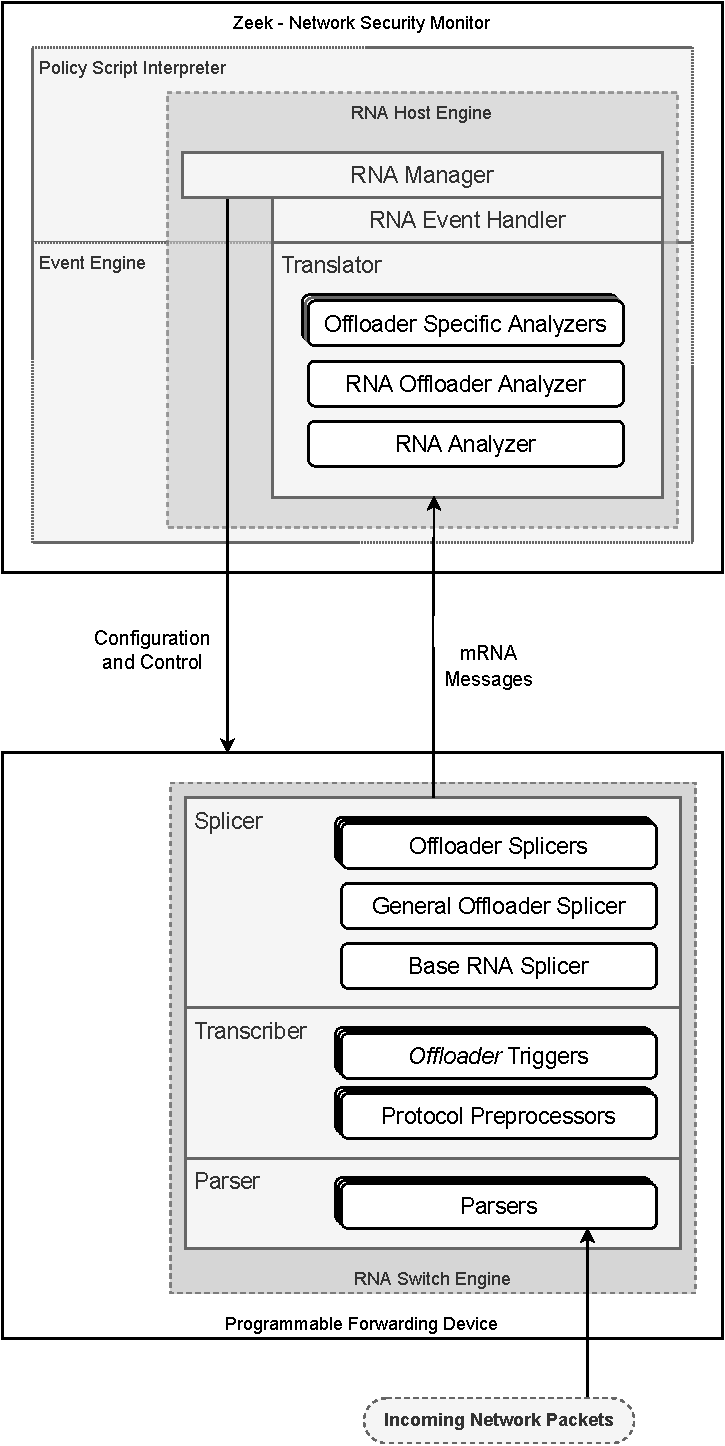
\includegraphics[width=0.7\textwidth]{images/arch_low_level.pdf}  
    \end{center}
    \label{fig:arch_low_level}
    \legend{Source: the author}
\end{figure}

\subsection{Switch Engine}

As the packet arrives at the P4-switch, it is first processed by the programmable parser. The \textbf{RNA Parser} component is a state machine with all the parsers the \Offloaders{} may need. Each one extracts its headers from the packet, and forwards the payload to the next parser.

In our example which is shown in Figure \ref{fig:icmp_ex_parser}, the first parser would be the Ethernet parser, extracting its header, followed by the IPv4 and ICMP parsers. In the example figure, we also display other states of parsers that were not identified. When the Ethernet header is parsed, the next protocol is defined by the \texttt{ethertype} field, which in this case was the IPv4 protocol. The states and protocols displayed by dotted lines were possible protocols the deployment could parse, but since the packet was an ICMP, those parsers were not used.

\begin{figure}[ht]
    \caption{Parsing States - ICMP Parsing Example}
    \begin{center}
        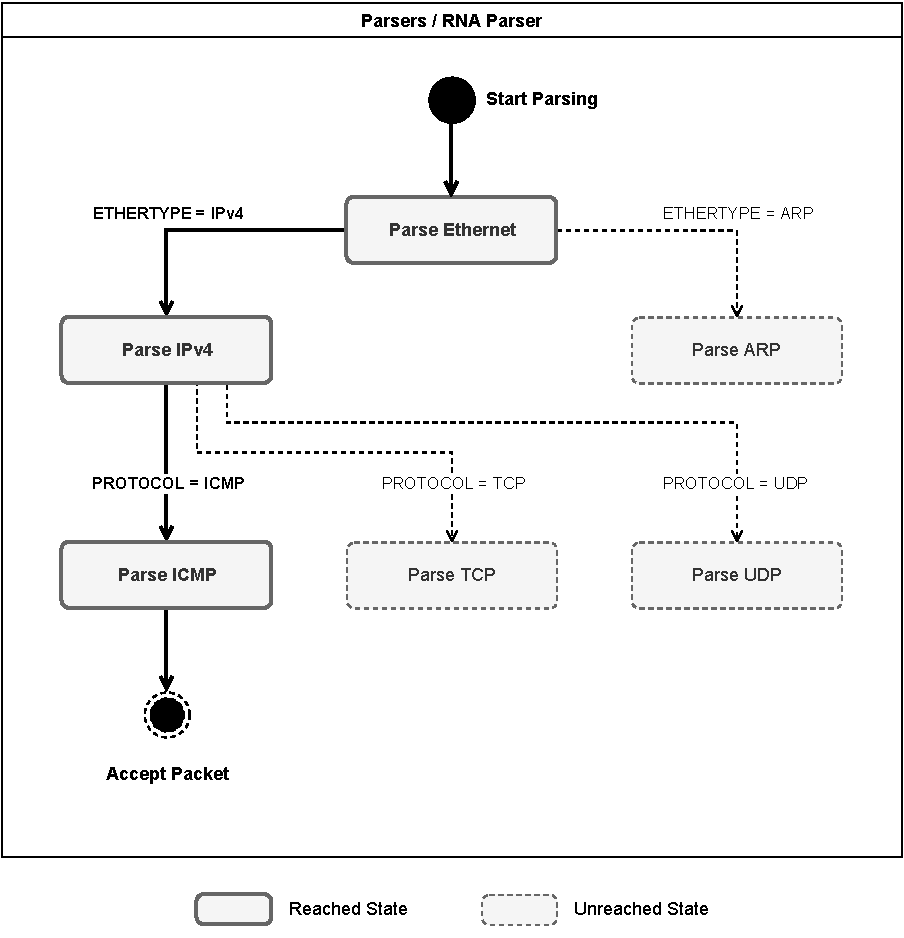
\includegraphics[width=0.7\textwidth]{images/icmp_ex_parser.pdf}  
    \end{center}
    \label{fig:icmp_ex_parser}
    \legend{Source: the author}
\end{figure}



The \textbf{RNA Transcriber} is the first component to be executed after the packets have their headers parsed, this happens in the ingress pipeline. In the Transcriber component, as shown in Figure \ref{fig:arch_low_level}, there are two types of modules, the Protocol Preprocessors and the Offloader Triggers, both of which may have multiple instances. We start explaining the Protocol Preprocessors since they are the first modules to be executed inside this component.

The Protocol Preprocessors are functions that every \ProtocolTemplate{} may execute to extract protocol metadata from the packet. This module is optional and every \ProtocolTemplate{} may have only one preprocessor. In our example, the processor extracts the ICMP type from the header and saves it in the metadata.

The next modules to be executed in the Transcriber are the Offloader Triggers, which are conditions that identify which \Offloader{} should be triggered. Each of these conditions is checked, and the first \Offloader{} to have its trigger condition valid is marked as the triggered one in the packet's metadata. In our example of an ICMP echo request, our trigger condition is \texttt{icmp.type = 8}. This ensures the \Offloader{} \textsc{ICMP Echo Request} is triggered when a ping packet arrives.

After a valid \Offloader{} is found, a copy of this packet is created and using this cloned packet, the switch will be able to construct the mRNA message. The original packet will follow its flow and be delivered to the originally intended destination. At this moment we transition into the Splicer component, where the construction of the summarized message starts. 

The \textbf{RNA Splicer} is executed after the packet leaves the ingress pipeline and it enters the egress pipeline\footnotemark{}. The RNA Splicer is composed of the two following types of splicers:

\begin{itemize}
    \item The \textbf{RNA Base Splicer} constructs the base header for the mRNA message. This header contains general information, which all \Offloaders{} can use. This includes, for example, source IP, destination IP, L3, and L4 protocols. In our example, the RNA Base Splicer sets both source and destination IPs, the L3 protocol to \texttt{IPv4}, and L4 protocol to \texttt{ICMP}. The Base Splicer is executed for every triggered \Offloader{}.
    
    \item The \textbf{Offloader Splicers} are splicers that every \Offloader{} may have. Each \Offloader{} Splicer constructs the header with the extra information required to execute its functionality. In our example, the \textsc{ICMP Echo Request} Splicer will construct a header with information about the ICMP packet: \texttt{type}, \texttt{code}, \texttt{sequence}, and \texttt{id}.
\end{itemize}

\footnotetext{Since we are explaining the architecture behind \TheSolutionName{}, we are not considering the inner workings of the programmable data plane, where a buffer connects the ingress and egress pipeline.}

After every Splicer has finished constructing their headers, the mRNA message will be ready. The payload and headers, which together form the mRNA, are then merged and sent to Zeek's monitoring interface, effectively finishing the processing on the Switch Engine. From now on, Zeek's Translators will work to support the monitoring infrastructure.

\subsection{Host Engine}

In the this section, we describe how the Host Engine receives the mRNA messages and uses them to execute the monitoring scripts. Figure \ref{fig:arch_low_level} shows the first components to receive the mRNA message are the Translators. In Zeek's architecture there is one module responsible for analyzing each protocol, which are called Analyzers. Every Analyzer parses their respective headers and forwards the payload to the next one.

The first Analyzer to receive the mRNA message is not displayed in Figure \ref{fig:arch_low_level} and is executed before the RNA Analyzer. Since the mRNA message is built over the Ethernet protocol, the first analyzer to receive the message is the Ethernet Analyzer. This Analyzer, using the \texttt{ethertype} code, forwards then every received packet to the Analyzer responsible for parsing the next protocol layer.




\section{Code Generation}
        % 10 (or 20 if no implementation chapter)
\chapter{Implementation}
\label{cap:implementation}

% 
% This chapter is possibly too small to be a chapter... maybe will be merged with evaluation 
%
  % 10
\chapter{Proof of Concept and Evaluation}
\label{cap:evaluation}

In this chapter, we present how the automatic code generation mechanism proposed in \autoref{cap:code_gen} was implemented in a fully functional proof of concept. We also describe how we evaluated the gains in performance and ease of development and deployment for users of our framework.

To facilitate the development of this project and to keep the scope within a defined limit, we did not use P4-compatible hardware. Instead, we used the Behavioral Model version 2 (BMv2) software-based switch \cite{BMv2} to run the P4 code. This enabled us to develop with high agility the generation tool and to test the development more frequently, making sure the prototype was functional.

% ==============================================================================
%                               IMPLEMENTATION
% ==============================================================================

\section{Prototype Implementation and Deployment}
\label{sec:evaluation:implementation}

In this section, we describe some implementation details of the code generation mechanism that were not previously discussed. We divide this explanation into three subsections. We first explain the structure of the Protocol and Offloader Templates, which are two of the main inputs for our mechanism. Then we explain some of the implementation aspects of our prototype. To finalize, we explain how the output of our mechanism, the automatically generated code, is deployed in a virtualized network with an emulated P4 switch.


\subsection{Protocol and Offloader Templates}

The Protocol and Offloader Templates have a similar structure based on a configuration file. This configuration file is in the Hjson \cite{Hjson} format, which is based on the well-known JSON format. We first explain the Protocol Templates using the example configuration shown in \autoref{fig:icmp_template:config}. Each Protocol Template needs to provide header definitions so it may be parsed. This is done by providing the name of the header structure and the file where it was defined (lines 13 and 12). The protocols may optionally have a custom \textit{ingress processor} and a custom parser to enable parsing of variable-size headers, both of which were explained in \autoref{sec:rna:detailed_design}.

\begin{figure}[htb]
    \caption{Template configuration file: \texttt{icmp.hjson}}
    \begin{center}
        \lstinputlisting[style=hjson]{code/icmp_template/icmp.hjson.txt}
    \end{center}
    \label{fig:icmp_template:config}
    \legend{Source: the author (2022).}
\end{figure}

To enable a Protocol Template to be linked to its children, we need to define the parameter called \texttt{next\_protocol\_selector}. It specifies the field of the protocol header that will be used to select the next protocol (line 15). To link the protocol to its parent, we need to specify the parent protocol identifier (line 7) and specify what value the \texttt{next\_protocol\_selector} parameter must have for the packet to be forwarded to the child protocol (line 8). With this structure, the mechanism is able to generate all required code for parsing the protocols in the Switch Engine.

An Offloader Template is also based on a configuration file, and we use \autoref{fig:icmp_echo:config} as an example. Each Offloader needs to be associated with a Protocol Template by its identifier (line 5). Each Offloader then must have a header structure definition (line 8) for its mRNA message. This header structure is defined in a P4 file, which is also a part of the template, and its path must be specified in the configuration (line 9). The rest of the parameters used for the Switch Engine are extracted from separate P4 files, the splicer, and the trigger condition (lines 10 and 11). For the Host Engine, the template must specify the C++ code and header files, as well as the name and \textit{namespace} of the Analyzer (lines 14 to 22). To finalize, the configuration also specifies what Zeek Events the Offloader is capable of offloading (lines 23 to 26).

\begin{figure}[htb]
    \caption{Template configuration file: \texttt{icmp\_echo\_message.hjson}}
    \begin{center}
        \lstinputlisting[style=hjson]{code/offloader_template/icmp_echo_message.hjson.txt}
    \end{center}
    \label{fig:icmp_echo:config}
    \legend{Source: the author (2022).}
\end{figure}

\subsection{Prototype Implementation}

Our prototype implementation of the code generation mechanism follows all architectural details explained in Chapters \ref{cap:rna} and \ref{cap:code_gen}. It was implemented in Python 3 in a modular way so it could be maintained and further developed as the RNA Framework grows. To explain further details of the implementation that were not yet discussed, we follow the same structure used to explain the mechanism details in \autoref{sec:code_gen:detailed}, and we start with the Event Extraction part.

The Event Extraction component was a strong reason for choosing Python as our programming language since Zeek provides its own Python library for parsing Zeek Scripts. In this component, we parse the provided Zeek Scripts and search their Abstract Syntax Tree (AST) for event handler declarations. Once those handler declarations are found, we extract their identifiers and forward this list of identifiers to the next component, the Knowledge Model Builder.

The Knowledge Model Builder uses as inputs the templates and the Zeek Script events. In this component, we create a graph structure following \autoref{alg:build_graph} and the procedures explained in \autoref{sec:code_gen:detailed}. In our implementation, we use exceptions to handle the flow of the algorithm and abort when any requirements are not met. Since our implementation of the Knowledge Model Builder does not differ from the algorithm explained in \autoref{sec:code_gen:detailed}, we do not repeat the explanation in this section.

\vspace{1em}

The Code Generation component in our prototype uses template files with markers to insert the generated code in the correct location. The files used for this purpose are called \textit{master template} files, and this is what defines the structure and organization of the output of our mechanism. In the \textit{master template}, markers are predefined strings in specific formats that indicate where a specific code section will be inserted. To generate code that will replace these markers, we use a structure similar to an AST, where each code element is a node, implemented using a class containing its children nodes. The mechanism first builds this structure, linking all nodes, then converts the root node to a string. This conversion is done recursively for each node, returning, in the end, the complete generated code. When the code is generated, we replace the corresponding marker with the generated code and save the file to the output directory.

The output of our mechanism is also composed of code that is provided with each template. To merge these provided sections of code, we use the same strategy as explained in the previous paragraph. We use template files with markers to define where each part of the code will be inserted. We also split some files, mainly on the Zeek Script, as \textit{no-edit} files. These \textit{no-edit} files are copied to the output location unaltered because they do not need any modifications, and some of them are static files required by the Zeek Package structure.

When our mechanism is executed, it generates an output folder containing all the automatically generated code. As explained in the previous chapter, we have not yet implemented the deployment of the P4 code using the Zeek Package, so we split this output folder into two sub-folders. One of the folders contains the P4 code for the switch, and one contains the Zeek Plugin package. In the next section, we explain how the P4 code and the Zeek Plugin are deployed.

\subsection{RNA Deployment}
\label{sec:evaluation:deployment}

The deployment of the RNA framework takes place in a virtualized network and uses an emulated P4 switch, so no specific hardware or Programmable Forwarding Devices (PFDs) are required to test our approach. To emulate the switch, we use the \textit{p4app} tool, which sets up a virtualized network and instantiates a BMv2 switch \cite{BMv2} within a Docker container. The \textit{p4app} tool \cite{P4App} compiles the P4 code and loads it into an emulated programmable forwarding device. To set up the network, \textit{p4app} uses a tool called \textit{mininet} \cite{Mininet}, which creates all the interfaces for each of our devices (hosts and switches) and allows us to simulate different network topologies. To run Zeek, we use a custom Docker image that contains all required dependencies. When executing Zeek, we link this Docker container's network to the \textit{p4app} container network, which allows us to run Zeek on any interface of the virtual switch, but, usually, on the port setup as a mirroring port.

In our tests, we used a simple topology with two hosts linked by an emulated P4 switch, with a mirroring port where Zeek is listening. The mRNA messages generated by the switch are sent to the mirroring port, where Zeek is listening for incoming packets. To generate the traffic that is analyzed by our mechanism, we used two different methods. The first method is using \textit{p4app} to open terminals in virtual hosts, where we are able to run programs and generate traffic for the framework to process. The second method is using packet traces that were previously captured and forwarding these traces to be processed as incoming traffic.

% ==============================================================================
%                                EVALUATION
% ==============================================================================

\section{Evaluation}
\label{sec:evaluation:evaluation}

We now present the evaluation of our proposed approach, both the RNA framework and the automatic code generation mechanism. We assess the ability of our code generator to generate correct code and how it enables an inexperienced network operator to offload monitoring scripts to PDPs. Last, we assess the performance of the output of our solution, the automatically generated instance of the RNA framework. These aspects can be formalized as the following research questions (RQs):

\begin{itemize}
    \item \textit{RQ1}: Is the code generator mechanism able to correctly generate code to offload a set of Zeek Scripts using RNA?
    
    \item \textit{RQ2}: How many lines of code did the code generator yield? And how many extra lines would a developer or network operator need to code to deploy the solution?
    
    \item \textit{RQ3}: How does the performance of a Zeek deployment with RNA compare to a deployment without RNA?
\end{itemize}

To answer those questions, we deploy an automatically generated instance of RNA and test it using traces containing attacks that trigger warnings on a set of predefined scripts. To limit the scope of this project, we decided that the supported scripts should \textit{(1) not require any state management by the generated RNA code} and should \textit{(2) not require any stream reassembly}. Those scripts are:

\begin{itemize}
    \item \textit{FTP Bruteforcing}: This script detects FTP authentication brute-force attacks. It triggers a warning after a number of unsuccessful login attempts by an FTP client.
    \item \textit{Detect traceroute}: Detects trace-route attempts by monitoring \textit{ICMP Time Exceeded} messages. This script is provided by Zeek, and originally it uses \textit{Signature Detection} \cite{ZeekSignatureFramework}. Since we do not support this feature on RNA, we disabled the usage of \textit{signatures} on this script.
    \item \textit{ICMP Pingback}: Developed by \citeonline{CorelightPingback}, it detects the usage of ICMP ping tunnels created by the Pingback C2 tool.
    \item \textit{NTP Monlist}: This script detects NTP Monlist attacks \cite{NtpMonlist}.
\end{itemize}


\subsection{Experiment Workload and Dataset} % Workload?

The workload used for our experiments was a combination of a legitimate dataset with an attack dataset, some of which were generated by us. The legitimate dataset used was the \textit{CAIDA Anonymized Internet Traces 2016} \cite{CAIDA2016}, which comes from a high throughput backbone. Since this packet trace was too big, we selected only a small (but dense) ten-second window to use for our experiments, which we now refer to as our \textit{legitimate dataset}. This packet trace was then merged with smaller well-known attack traces, whose combination we call \textit{attacks dataset}, with $1200$ packets. Combining these two traces ensures our selected scripts trigger warnings. This combined dataset is the one used for our experiments, which we refer to as the \textit{combined dataset}. The workload has $5.5$ million packets, a mean of $556$ thousand packets per second (kpps) and $3269$ megabits per second (Mbps). \autoref{fig:pps_in_time} shows the variation of packets per second (pps) for our dataset, as well as the placement of the attacks used.

% Add attack traces statistics or remove plot: characterize dataset
\begin{figure}[H]
    \caption{Packets Per Second (pps) for the dataset}
    \begin{center}
        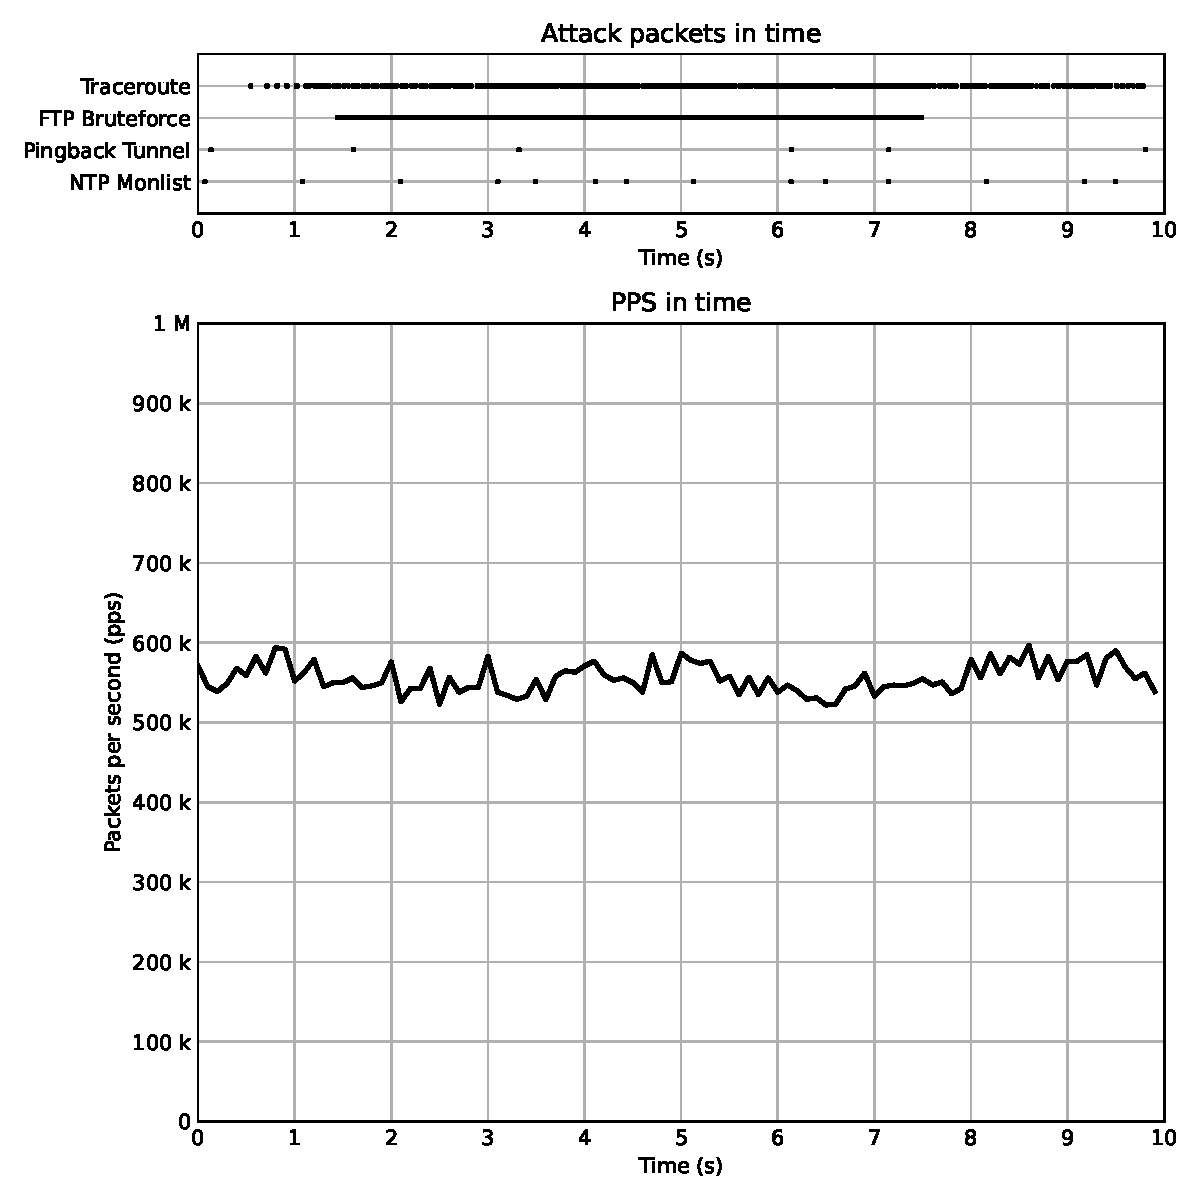
\includegraphics[width=0.7\textwidth]{images/pps_in_time.pdf}  
    \end{center}
    \label{fig:pps_in_time}
    \legend{Source: the author (2022).}
\end{figure}

% Explain the dataset (with plots) + attacks + ferramentas para gerar dataset
% - datasets status: taxa de pico, pps, total size, duration, packets, characteristics...
% - Attacks:
% - FTP Bruteforcing
% - Pingback https://github.com/corelight/pingback
% - Detect traceroute
% - NTP Monlist



\subsection{Experiment setup and methodology}
\label{sec:evaluation:setup}

In this section, we describe the setup of our experiment. The experiment used the same technologies described in \autoref{sec:evaluation:deployment}, relying on network virtualization, P4 emulation to run our switch, and containerization to run Zeek. The objective of our evaluation was to compare the functionality and performance of the Zeek Scripts without RNA compared with RNA.

Switch emulation does not perform as fast as a real P4 hardware switch, which makes it impossible for us to execute our experiment with a P4 switch in real-time since we only use emulated switches. In this scenario, the emulated switch would become a bottleneck, preventing the traffic from reaching Zeek at the same rate as it enters the P4 pipeline. For this reason, we assess only the performance of the Zeek monitoring system. We assume that a (hardware) programmable forwarding device would be able to execute the program at line rate if the provided program fits the device's memory.

\vspace{1em}

To overcome the performance deficit of emulated P4 switches, we process the combined dataset before running the experiment, effectively creating a second dataset. This second dataset represents a real-world output of a P4-switch, receiving our combined dataset and processing it at line rate. We call this second dataset the \textit{RNA dataset}.

To explain the generation of this second dataset, we use \autoref{fig:rna_dataset_diagram}. The first step is to select from our dataset only the packets that may trigger an Offloader, which will eventually generate an mRNA message. With this intermediate trace, we execute our emulated P4 switch, which is now able to process the dataset faster due to the decreased amount of traffic. This results in a dataset with only mRNA messages, the \textit{RNA dataset}. It is also important to note that in all datasets during this process, all packets have their timestamps preserved, and real behavior is emulated.

\begin{figure}[htb]
    \caption{RNA dataset creation diagram}
    \begin{center}
        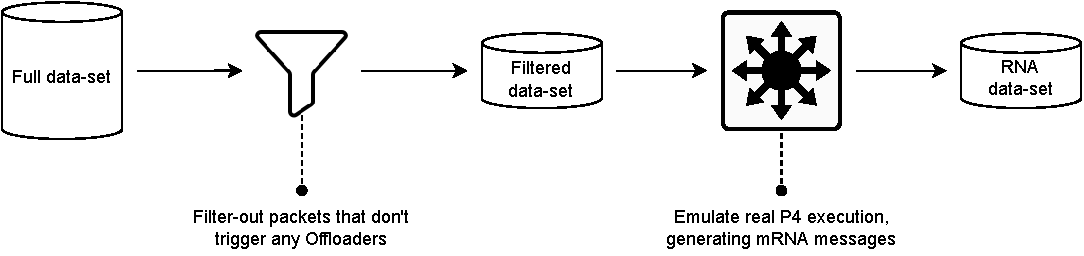
\includegraphics[width=1.0\textwidth]{images/rna_dataset_creation.pdf}  
    \end{center}
    \label{fig:rna_dataset_diagram}
    \legend{Source: the author (2022).}
\end{figure}

Now that we have our two datasets, the \textit{combined dataset} and the \textit{RNA dataset}, we need to execute Zeek in both scenarios and compare its output and performance. This is done by running Zeek in a Docker container connected to the host computer by a virtual network interface. In this network interface, we replay those two traces, one at a time, and record the memory and CPU usage. Each scenario was executed fifteen times to account for variability. The experiments were executed on a notebook with an Intel Core i9-10885H (\SI{5.3}{GHz}, 8 cores, 16 threads) CPU, \SI{16}{GB} ($2 \times$\SI{8}{GB}) of DDR4 RAM (\SI{3200}{MT/s}), and a \SI{1}{TB} NVMe SSD. While the experiments were executed, in order not to affect the results, no other non-essential services were executed on the computer.

% Methodology?

% \subsection{Methodology}

% Explain results
% - accuracy
%   + script count
% - development cost savings (and less prone to development mistakes)
%   - Show table with multiple combinations of scripts: [1], [2], [3], [4], [1, 2, 3, 4]
% - performance gain
%   - memory, cpu, (execution time/detection time)


\subsection{Results}

In this section, we describe the results of the experiment and functional assessment of our code generation mechanism. We first present the functional results, answering research questions one (RQ1) and two (RQ2). We later present the performance results, answering \textit{RQ3}.

\subsubsection*{Functional results}

To assess whether our proposed mechanism works, we used our prototype and the attacks dataset to compare the output of a Zeek deployment with and without RNA. After executing both setups and comparing the output of Zeek's \textit{notices}, we concluded that our code generation mechanism was able to generate code to successfully offload four different scripts, namely \textit{FTP Bruteforcing}, \textit{Detect traceroute}, \textit{ICMP Pingback}, and \textit{NTP Monlist}. All of these scripts were able to detect, with complete accuracy, all the attacks present in the workload of the experiment, resulting in no difference between the execution with and without RNA in terms of detection.

To answer the second question, we manually inspect the generated code for RNA. Our objective is to check whether our approach is helpful and facilitates the deployment of RNA. \autoref{tab:lines_per_script_count} summarizes the main results obtained. The generated output instance of RNA for offloading our four Zeek Scripts (described above in this section) has $2967$ lines of code. To develop a new Protocol Template, according to \autoref{tab:lines_by_protocol_template}, a median of $40$ lines of code would need to be written, and for a new Offloader Template (\autoref{tab:lines_by_offloader_template}), a median of $224$. This gives developers a big advantage over writing a fully standalone solution since templates are small and easier to maintain than a complete solution. The main advantage leans on the reuse of Protocol and Offloader Templates. Using templates, a network operator is able to deploy RNA without writing a single line of code, only with a command. The automatic code generator identifies the needed events to offload the desired scripts and generates the complete code.


\begin{table}[htb]
    \caption{Lines of Code per Script Count}
    \begin{center}
        \begin{tabular}{|l|r|}
            \hline
            \textbf{Monitoring Script Count} & \multicolumn{1}{l|}{\textbf{Generated Lines Median}} \\ \hline
            1 Monitoring Script              & 2113.5                                             \\ \hline
            2 Monitoring Scripts             & 2421.5                                             \\ \hline
            3 Monitoring Scripts             & 2714.0                                             \\ \hline
            4 Monitoring Scripts             & 2967.0                                             \\ \hline
        \end{tabular}%
    \end{center}
    \label{tab:lines_per_script_count}
    \legend{Source: the author (2022).}
\end{table}

\begin{table}[htb]
    \caption{Lines of code of Protocol Templates}
    \begin{center}
        \begin{tabular}{|l|r|r|r|}
            \hline
            \textbf{Protocol Template} & \multicolumn{1}{l|}{\textbf{Lines of Configuration}} & \multicolumn{1}{l|}{\textbf{Lines of code}} & \multicolumn{1}{l|}{\textbf{Total Lines}} \\ \hline
            Ethernet Protocol          & 13                                                   & 13                                          & 26                                        \\ \hline
            IPv4 Protocol              & 17                                                   & 26                                          & 43                                        \\ \hline
            IPv6 Protocol              & 17                                                   & 20                                          & 37                                        \\ \hline
            ICMP Protocol\footnotemark & 59                                                   & 77                                          & 136                                       \\ \hline
            TCP Protocol               & 22                                                   & 45                                          & 67                                        \\ \hline
            UDP Protocol               & 21                                                   & 10                                          & 31                                        \\ \hline
            \textit{Total}             & \textit{149}                                         & \textit{191}                                & \textit{340}                              \\ \hline
            \textit{Median}            & \textit{19}                                          & \textit{23}                                 & \textit{40}                               \\ \hline
        \end{tabular}%
    \end{center}
    \footnotetext{TODO}
    \label{tab:lines_by_protocol_template}
    \legend{Source: the author (2022).}
\end{table}

\begin{table}[htb]
    \caption{Lines of code of Offloader Templates}
    \begin{center}
        \begin{tabular}{|l|r|r|r|}
            \hline
            \textbf{Offloader Template}        & \multicolumn{1}{l|}{\textbf{Lines of Configuration}} & \multicolumn{1}{l|}{\textbf{Lines of code}} & \multicolumn{1}{l|}{\textbf{Total Lines}} \\ \hline
            NTP Message                        & 27                                                   & 152                                         & 179                                       \\ \hline
            ICMP Echo Message                  & 28                                                   & 157                                         & 185                                       \\ \hline
            ICMP Time Exceeded & 28                                                   & 305                                         & 333                                       \\ \hline
            FTP Request and Reply              & 28                                                   & 235                                         & 263                                       \\ \hline
            \textit{Total}                     & \textit{111}                                         & \textit{849}                                & \textit{960}                              \\ \hline
            \textit{Median}                    & \textit{28}                                          & \textit{196}                                & \textit{224}                              \\ \hline
        \end{tabular}%
    \end{center}
    \label{tab:lines_by_offloader_template}
    \legend{Source: the author (2022).}
\end{table}


% \begin{figure}[htb]
%     \caption{Generated lines per script count}
%     \begin{center}
%         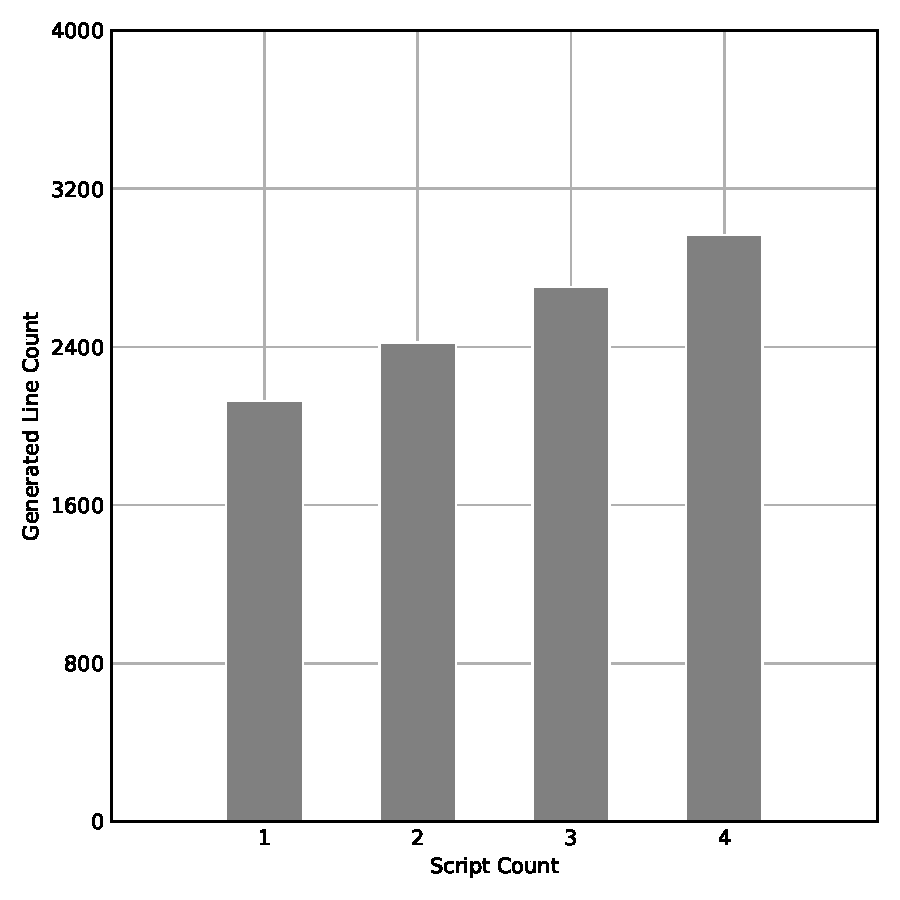
\includegraphics[width=0.7\textwidth]{images/generated_lines.pdf}  
%     \end{center}
%     \label{fig:gen_lines_per_script}
%     \legend{Source: the author (2022).}
% \end{figure}


\subsubsection*{Performance results}

To answer our third research question and assess the performance gain of offloading scripts with RNA, we replayed both of our datasets, the \textit{combined dataset}, and the \textit{RNA dataset}. When replaying the RNA dataset, we enabled our Zeek Plugin, which processed the incoming mRNA messages. This resulted in a significant gain in performance. As Figure \ref{fig:rna_perf} shows, the mean CPU\footnote{Usage of one CPU core. $100\%$ represents usage of a full core, $150\%$ represents usage of one and a half CPU cores.} usage without RNA is $109\%$, and memory usage reaches a maximum of $960.64$ MB by the end of the experiment. With RNA (simulated by using the \textit{RNA dataset}), mean CPU utilization was $1.9\%$ and the maximum memory usage was $235.07$ MB. Additionally, without RNA, a mean of $35.24\%$ of the packets was dropped. The high dropped packet rate resulted in one of the attacks, the \textit{FTP Bruteforce Attack}, not being detected in $93.3\%$ of the iterations executed without RNA. Using our approach, no packets were dropped, and all attacks were detected in all executions of the experiment.

In \autoref{fig:rna_perf}, at time \SI{5}{s}, we observe a significant change in the increase of memory and CPU usage. Our hypothesis is that this is the moment internal Zeek buffers are filled, decreasing the rate packets are read, slowing down the increase of memory usage, and increasing the CPU usage. In a real-world scenario, network operators would not allow an IDS to drop packets and would increase the processing power or implement a sampling strategy. Our intention with this comparison is to contrast the usage of a normal Zeek deployment compared to our RNA framework, which uses Programmable Data Planes to offload IDS operations. Nevertheless, our results suggest that the observed reduction in CPU usage for the RNA-based setup would allow for the use of a smaller cluster for the given scenario. 

Another important note is that the Dynamic Protocol Detection (DPD), which we presented in \autoref{sec:bg:zeek_ee}, is unable to dynamically detect protocols when RNA is used, potentially resulting in better performance, giving RNA an advantage. This is also one of the assumptions we made to simplify the development of the mechanism.

% Metrics:
% 1. How many scripts we can run (without intervention)
% 2. How many lines were produced per script
%     a. Include copied from the template (maybe create a table with the outline)
% 3. Performance gain in offloading (optional): compare a raw data set vs mRNA messages data set.
%     a. memory, cpu, execution time

\begin{figure}[htb]
    \caption{RNA Performance Evaluation}
    \begin{subfigure}{.5\textwidth}
        \centering
        \vspace{1em}
        \caption{CPU usage by time}
        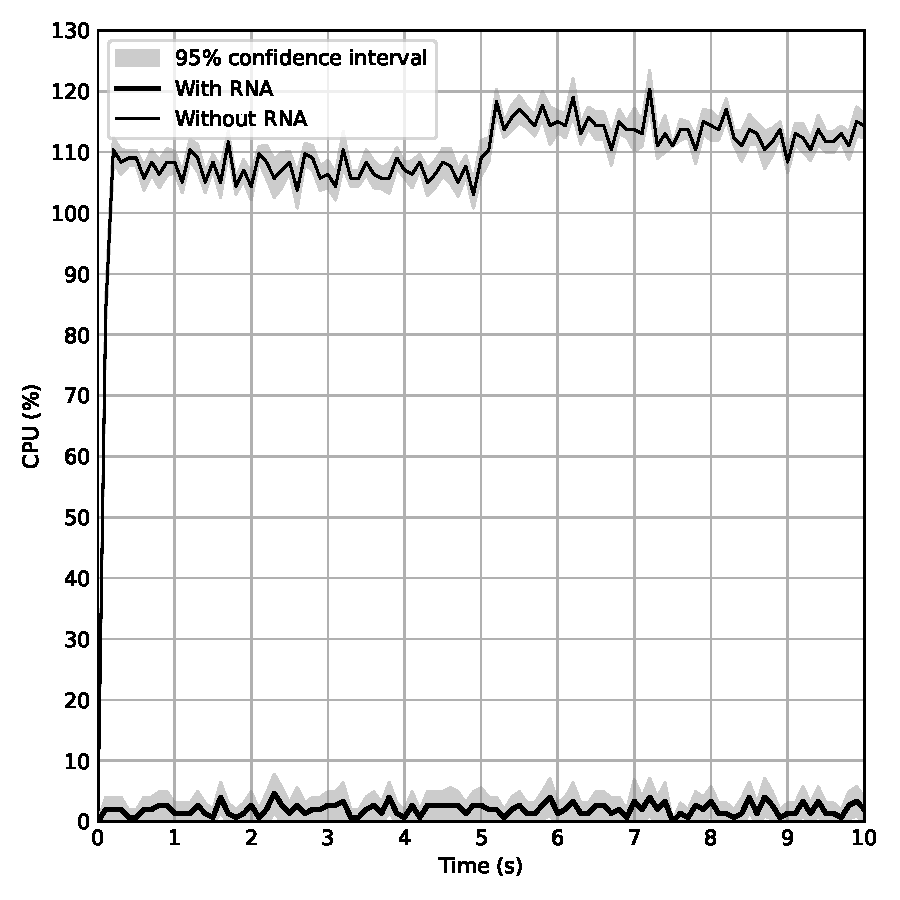
\includegraphics[width=1.0\textwidth]{images/aggregated_cpu_plot.pdf}
        \label{fig:rna_cpu}
    \end{subfigure}%
    \begin{subfigure}{.5\textwidth}
        \centering
        \vspace{1em}
        \caption{Memory usage by time}
        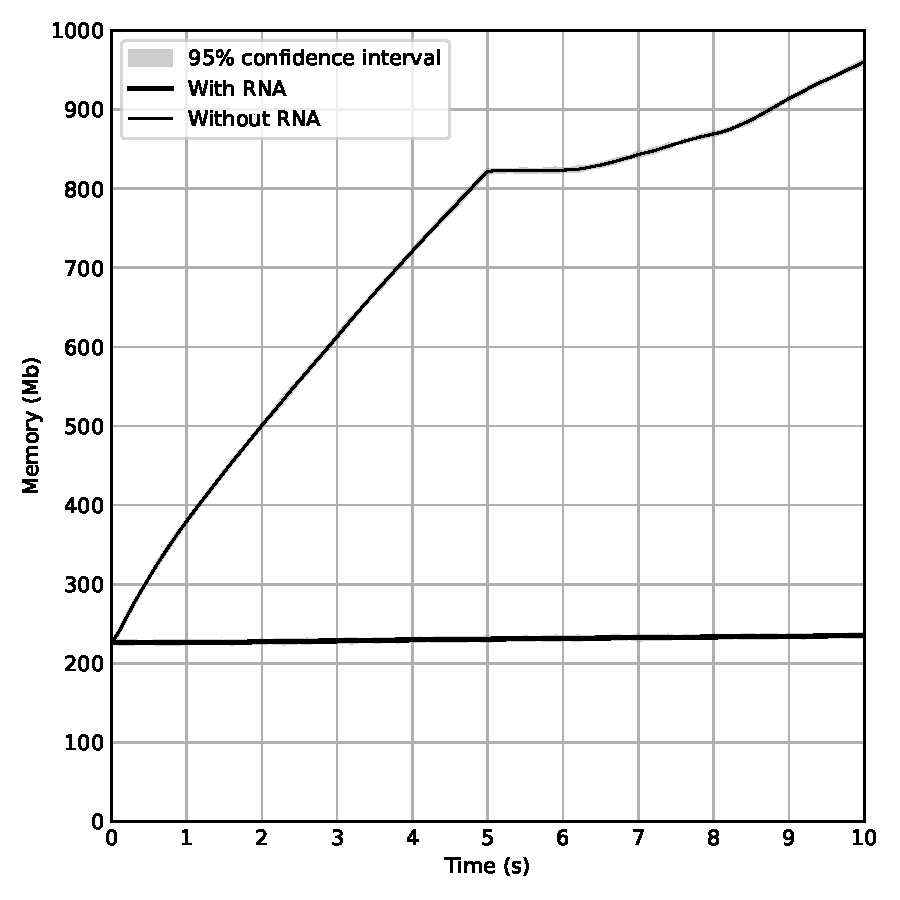
\includegraphics[width=1.0\textwidth]{images/aggregated_memory_plot.pdf}
        \label{fig:rna_mem}
    \end{subfigure}
    \label{fig:rna_perf}
    \legend{Source: the author (2022).}
\end{figure}

% 
% ====================       Pode revisar até aqui :)       ====================
% 
      % 5
\section{Conclusion and Future Work} 
\label{sec:conclusion}

% 1,5 columns.

\blindtext[7]

      % 1

\bibliographystyle{abntex2-alf}
\bibliography{biblio}

\end{document}
